\documentclass[17pt]{beamer}
\usepackage{tikz}
\usepackage{outlines}
\usepackage{hyperref}


\usetheme{Berlin}
\usecolortheme{default}


\title[Preproject Presentation] %optional
{Canvas Quiz Previewer}
\subtitle{Preproject - Ideas and Objectives}
\author[Cheng, Shi] % (optional)
{J.~Cheng\inst{1} \and C.~Shi\inst{1}}

\institute[U Mich] % (optional)
{
  \inst{1}%
  Graduate Students\\
  Department of ECE\\
  University of Michigan
}

\date[\today] % (optional)
{EECS-551, December 2021}

% Use a simple TikZ graphic to show where the logo is positioned
% \logo{\begin{tikzpicture}
% \filldraw[color=red!50, fill=red!25, very thick](0,0) circle (0.5);
% \node[draw,color=white] at (0,0) {LOGO HERE};
% \end{tikzpicture}}
\begin{document}
\frame{\titlepage}
%Highlighting text

\begin{frame}
    \frametitle{Table of Contents}
    \tableofcontents
\end{frame}

\section{Objectives}
\begin{frame}
    \frametitle{Objectives}
    \begin{outline}
        \1 Create a simple software to visualize the canvas quiz
        \1 Required output of the software
            \2 .txt file for canvas upload
            \2 .tex file for \LaTeX \: compilation
    \end{outline}
\end{frame}

\section{Approach}
\begin{frame}
    \frametitle{Approach - conversions}
    \begin{itemize}
        \item host a small GUI using web browser - for edit and preview
        \item using \href{https://github.com/trentm/python-markdown2}{markdown2} to convert the markdown style questions to html
        \item using \href{https://github.com/rufuspollock/markdown2latex}{markdown2latex} to convert the markdown to latex
        
    \end{itemize}
\end{frame}

\begin{frame}
    \frametitle{Approach - Implementation details}
    \begin{itemize}
        \item website will be hosted by individual students 
        \item Python file compiled to a single executable file
        \item student launch website by double click the executable file
        \item website hosted on localhost by students
    \end{itemize}
\end{frame}

\section{Preliminary Design}
\begin{frame}
    \frametitle{Preliminary Design}
    \begin{figure}
        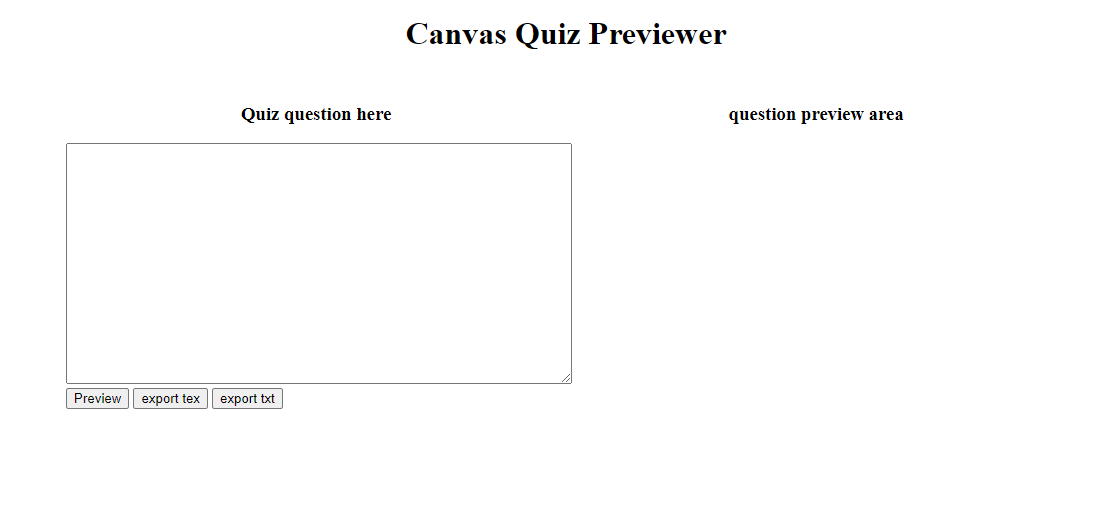
\includegraphics[width=0.8\textwidth]{img/prelim_design.png}
        \caption{Preliminary Design}
    \end{figure}
    % This is an preliminary design for the user interface.
\end{frame}

\section{Potential Improvements}
\begin{frame}
    \frametitle{Potential Improvements}
    Related Chapter Detector \\
    finding the latest chapter of the class that is related to the quiz question
\end{frame}

\begin{frame}
    \frametitle{Implementation details}
    \begin{itemize}
        \item extablish pre-extracted keywords from each chapter
        \item extract keywords from the question
        \item come up with a scoring system for matching keywords
        \item potential opportunity to use \texttt{Subspace Learning} 
    \end{itemize}
\end{frame}

\section{end}
\begin{frame}
    \centering Canvas Quiz Previewer \\
    \begin{figure}
        
\includegraphics[width=30mm, scale=0.05]{img/canvas-preview-logo-large.png}
    \end{figure}
    University of Michigan \\
\end{frame}

\end{document}